% Digital Logic Report Template
% Created: 2020-01-10, John Miller

%==========================================================
%=========== Document Setup  ==============================

% Formatting defined by class file
\documentclass[11pt]{article}

% ---- Document formatting ----
\usepackage[margin=1in]{geometry}	% Narrower margins
\usepackage{booktabs}				% Nice formatting of tables
\usepackage{graphicx}				% Ability to include graphics

%\setlength\parindent{0pt}	% Do not indent first line of paragraphs 
\usepackage[parfill]{parskip}		% Line space b/w paragraphs
%	parfill option prevents last line of pgrph from being fully justified

% Parskip package adds too much space around titles, fix with this
\RequirePackage{titlesec}
\titlespacing\section{0pt}{8pt plus 4pt minus 2pt}{3pt plus 2pt minus 2pt}
\titlespacing\subsection{0pt}{4pt plus 4pt minus 2pt}{-2pt plus 2pt minus 2pt}
\titlespacing\subsubsection{0pt}{2pt plus 4pt minus 2pt}{-6pt plus 2pt minus 2pt}

% ---- Hyperlinks ----
\usepackage[colorlinks=true,urlcolor=blue]{hyperref}	% For URL's. Automatically links internal references.

% ---- Code listings ----
\usepackage{listings} 					% Nice code layout and inclusion
\usepackage[usenames,dvipsnames]{xcolor}	% Colors (needs to be defined before using colors)

% Define custom colors for listings
\definecolor{listinggray}{gray}{0.98}		% Listings background color
\definecolor{rulegray}{gray}{0.7}			% Listings rule/frame color

% Style for Verilog
\lstdefinestyle{Verilog}{
	language=Verilog,					% Verilog
	backgroundcolor=\color{listinggray},	% light gray background
	rulecolor=\color{blue}, 			% blue frame lines
	frame=tb,							% lines above & below
	linewidth=\columnwidth, 			% set line width
	basicstyle=\small\ttfamily,	% basic font style that is used for the code	
	breaklines=true, 					% allow breaking across columns/pages
	tabsize=3,							% set tab size
	commentstyle=\color{gray},	% comments in italic 
	stringstyle=\upshape,				% strings are printed in normal font
	showspaces=false,					% don't underscore spaces
}

% How to use: \Verilog[listing_options]{file}
\newcommand{\Verilog}[2][]{%
	\lstinputlisting[style=Verilog,#1]{#2}
}

\usepackage[section]{placeins}


%======================================================
%=========== Body  ====================================
\begin{document}

\title{ELC 2137 Lab 10: 7-segment Display with Time-Division Multiplexing}
\author{Aaron Mendoza}

\maketitle


\section*{Summary}

The purpose of this lab is to implement a clock-driven 4 digit display onto a Basys3 board using a counter module and previously built modules in other labs.

The first module built was a counter module. This is crucial to the lab because.... It has two inputs, clock and reset and outputs two of the most significant bits. In order to keep the counter going, it adds one to the previous value at every positive edge of the clock. Once all the bits hit 1, then the counter starts over at zero. 

The second module built was a wrapper that combined my seven segment display from lab 8 with the counter. The output of the counter becomes the input digit select of the seven segment display. I then generated this as a bitstream programmed it into my board to see if I chose the right number of bits, and since my seven segment display was not dim, I knew that 20 bits was the right number.

The third module built was a show 2's compliment module. This takes an input of 8 bits and outputs the two's compliment of that number in sixteen bits. If the data input is already positive, then the number is just passed to the output with zero's added to the left of the original bits. If the data input is negative, then the bits are flipped and 8 one's are added to the left of the original bits. The most significant bit of the data input is read to tell the program whether or not the number is positive or negative, outputting the sign of the input as well as the changed input or unchanged input by using a mux.

The final module built combined all of the modules together. The ALU from lab 9 takes in data and outputs it into the show2c module. The output of the show2c module goes into the data and sign inputs of the sseg4 module, whil the clk and reset inputs go into the counter module which controls the digits select of the sseg4 module. This was then programmed into my Basys3 board.


\section*{Results}


\subsection*{Simulation Waveforms}
\begin{figure}[ht]\centering
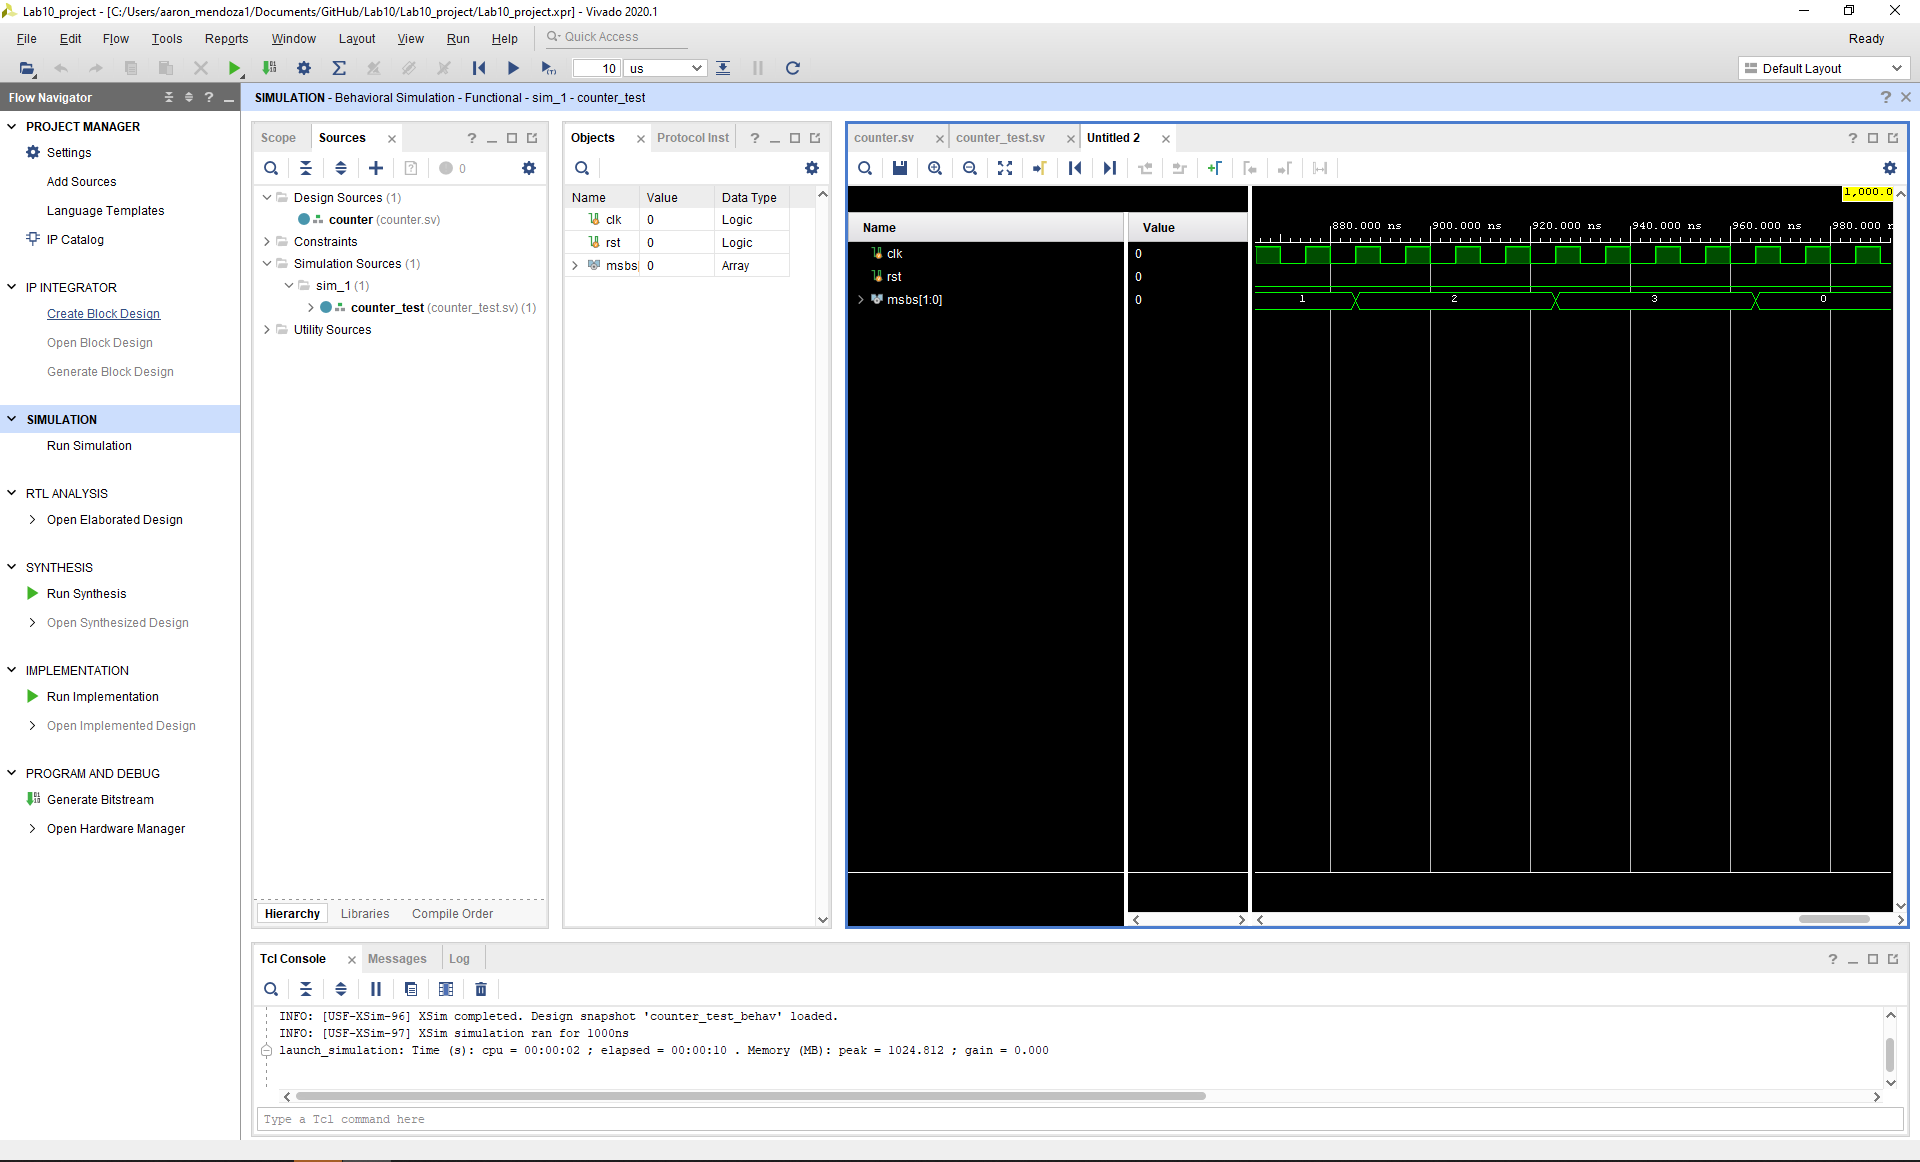
\includegraphics[width=1\textwidth,trim=19cm 15cm 0.5cm 4.5cm,clip]{counter_test_screenshot}
	\caption{Counter Simulation with N=4}
	\label{fig:sim_with_table}
\end{figure}


\begin{figure}[ht]\centering
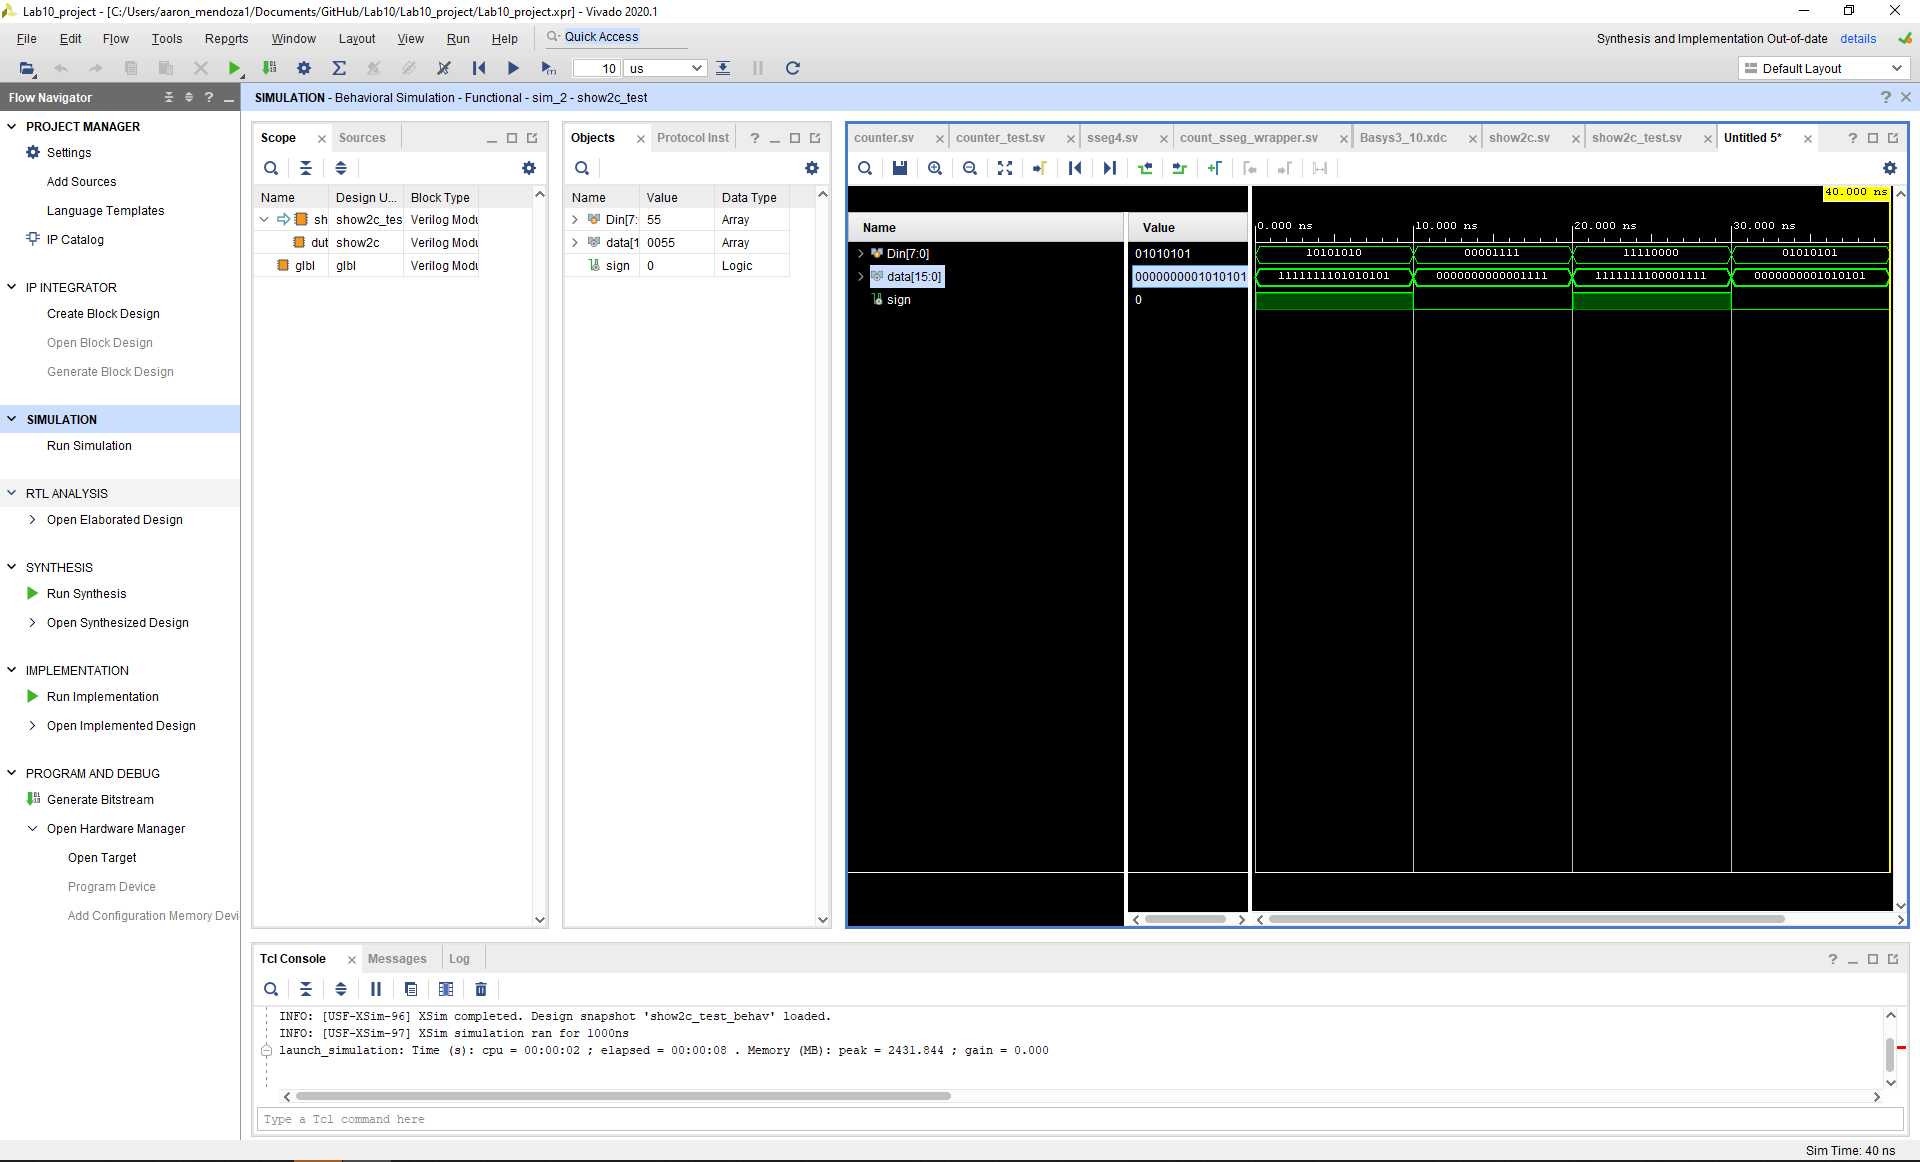
\includegraphics[width=1\textwidth,trim=19cm 15cm 0.5cm 4.5cm,clip]{show2c_test_screenshot}
	\caption{Show 2's Comp Simulation}
	\label{fig:sim_with_table}
\end{figure}

\FloatBarrier

\subsection*{Basys3 Board Pictures}
\begin{figure}[ht]\centering
\includegraphics[width=1\textwidth,trim=15cm 15cm 0.5cm 4.5cm,clip]{count_board}
	\caption{7-seg display after programming the count/sseg wrapper bitstream onto the Basys3 board}
	\label{fig:sim_with_table}
\end{figure}

\begin{figure}[ht]\centering
\includegraphics[width=1\textwidth,trim=15cm 15cm 0.5cm 4.5cm,clip]{pos_number}
	\caption{7-seg display after adding 16 and 9}
	\label{fig:sim_with_table}
\end{figure}


\begin{figure}[ht]\centering
\includegraphics[width=1\textwidth,trim=15cm 15cm 0.5cm 4.5cm,clip]{neg_number}
	\caption{7-seg display after subtracting 32 from 19}
	\label{fig:sim_with_table}
\end{figure}




\section*{Code}

\Verilog[firstline=22, lastline=41, caption=Counter Module Code]{Lab10_project/codedirectory/counter.sv}|

\Verilog[firstline=22, lastline=39, caption=Counter Test Module Code]{Lab10_project/codedirectory/counter_test.sv}|

\Verilog[firstline=22, lastline=48, caption=Counter 7-seg Module Code]{Lab10_project/codedirectory/count_sseg_wrapper.sv}|

\Verilog[firstline=22, lastline=51, caption=Show 2's Comp Module Code]{Lab10_project/codedirectory/show2c.sv}|

\Verilog[firstline=22, lastline=42, caption=Show 2's Comp Test Module Code]{Lab10_project/codedirectory/show2c_test.sv}|

\Verilog[firstline=22, lastline=67, caption=Top-Level Module Code]{Lab10_project/codedirectory/top_level.sv}|


\end{document}
